\documentclass[dvipsnames, hidelinks]{beamer}

% Enables the use of colour.
\usepackage{xcolor}
% Syntax high-lighting for code. Requires Python's pygments.
\usepackage{minted}
% Enables the use of umlauts and other accents.
\usepackage[utf8]{inputenc}
% Diagrams.
\usepackage{tikz}
% Settings for captions, such as sideways captions.
\usepackage{caption}
% Symbols for units, like degrees and ohms.
\usepackage{gensymb}
% Latin modern fonts - better looking than the defaults.
\usepackage{lmodern}
% Allows for columns spanning multiple rows in tables.
\usepackage{multirow}
% Better looking tables, including nicer borders.
\usepackage{booktabs}
% More math symbols.
\usepackage{amssymb}
% More math layouts, equation arrays, etc.
\usepackage{amsmath}
% More math fonts, like mathbb.
\usepackage{amsfonts}
% More theorem environments.
\usepackage{amsthm}
% More column formats for tables.
\usepackage{array}
% Adjust the sizes of box environments.
\usepackage{adjustbox}
% Better looking single quotes in verbatim and minted environments.
\usepackage{upquote}
% Better blank space decisions.
\usepackage{xspace}
% Better looking tikz trees.
\usepackage{forest}
% URLs.
\usepackage{hyperref}
% For plotting.
\usepackage{pgfplots}

% Various tikz libraries.
% For drawing mind maps.
\usetikzlibrary{mindmap}
% For adding shadows.
\usetikzlibrary{shadows}
% Extra arrows tips.
\usetikzlibrary{arrows.meta}
% Old arrows.
\usetikzlibrary{arrows}
% Automata.
\usetikzlibrary{automata}
% For more positioning options.
\usetikzlibrary{positioning}
% Creating chains of nodes on a line.
\usetikzlibrary{chains}
% Fitting node to contain set of coordinates.
\usetikzlibrary{fit}
% Extra shapes for drawing.
\usetikzlibrary{shapes}
% For markings on paths.
\usetikzlibrary{decorations.markings}
% For advanced calculations.
\usetikzlibrary{calc}

% GMIT colours.
\definecolor{gmitblue}{RGB}{20,134,225}
\definecolor{gmitred}{RGB}{220,20,60}
\definecolor{gmitgrey}{RGB}{67,67,67}

% Change some style options.
\usetheme{metropolis}
\usemintedstyle{manni}
\setbeamercolor{structure}{fg=gmitblue}
\setbeamercolor{frametitle}{fg=white, bg=gmitred}
\setbeamercolor{alerted text}{fg=gmitblue}
\usefonttheme[onlymath]{serif}

% \citeurl can be used to a clickable short url to a slide as a reference.
\renewcommand\footnoterule{}
\newcommand{\citeurl}[1]{\let\thefootnote\relax\footnotetext{\tiny \textcolor{gmitgrey}{\href{http://#1}{#1}}}}
\newcommand{\citeeg}[1]{\let\thefootnote\relax\footnotetext{\tiny \textcolor{gmitgrey}{#1}}}

% A basic horizontal rule.
\newcommand{\hr}{\rule{\textwidth}{0.5pt}}

% Prevent minted from showing errors.
\makeatletter
\expandafter\def\csname PYGdefault@tok@err\endcsname{\def\PYGdefault@bc##1{{\strut ##1}}}
\makeatother

\begin{document}
  \title{Fundamentals of functional programming}
  \subtitle{}
  \author{ian.mcloughlin@gmit.ie}
  \date{}

  \begin{frame}
    \titlepage
  \end{frame}

  \begin{frame}{Functional programming}
  \begin{center}
    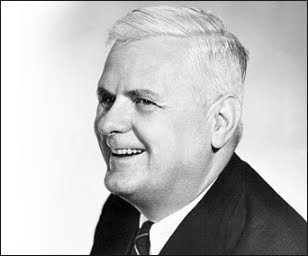
\includegraphics[height=1in]{img/church.jpg}
  \end{center}
  \begin{itemize}
    \item Functional programming is a programming paradigm.
    \item Alonzo Church introduced lambda calculus in 1932:
      $$ \lambda f . ( \lambda x . f ( x x ) ) ( \lambda . f ( x x ) )$$
    \item Functional programming is based on lambda calculus.
    \item Church was Turing's supervisor.
    \item Church--Turing thesis: lambda calculus \textbf{is} computation.
  \end{itemize}
\end{frame}

\begin{frame}{Imperative programming}
  \begin{center}
    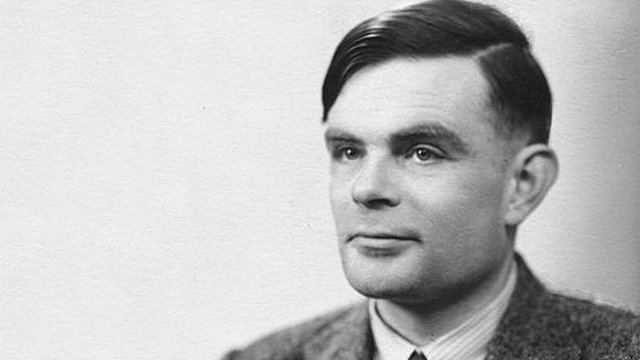
\includegraphics[height=1in]{img/alanturing.jpg}
  \end{center}
  \begin{itemize}
    \item Functional contrasts with imperative programming.
    \item C, Java, JavaScript are largely imperative.
    \item Programs have \textbf{state}, modified by \textbf{statements}.
    \item Origins in the Turing machine, a conceptual model created by Alan Turing.
    \item Turing machines and lambda calculus are equivalent.
  \end{itemize}
\end{frame}

\begin{frame}{von Neumann architecture}
  \begin{center}
    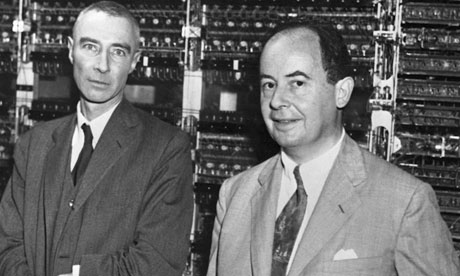
\includegraphics[height=1in]{img/vonneumann.jpg}
  \end{center}
  \begin{itemize}
    \item Modern computers largely based on the von Neumann architecture
    \item Designed in the main by John von Neumann.
    \item Key facet of von Neumann architecture is that data (state) and instructions (statements) are stored in the same memory space.
    \item Begs the question: \emph{what’s the difference between the 0’s and 1’s that mean stuff and the 0’s and 1’s that do stuff?}
  \end{itemize}
\end{frame}


\begin{frame}{Unsolvable problems}
  \begin{center}
    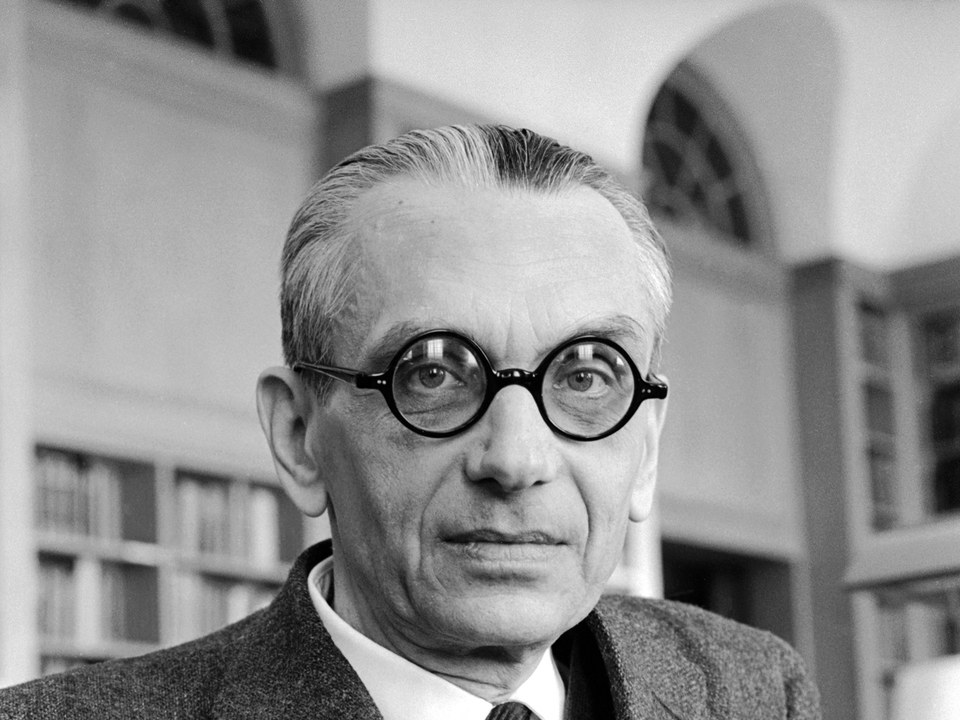
\includegraphics[height=1in]{img/godel.jpg}
  \end{center}
  \begin{itemize}
    \item Some problems are not solvable by any computer.
    \item Turing showed this with Turing machines, and Church with lambda Calculus.
    \item Worked on what’s come to be known as the Entscheidungsproblem, German for \textbf{decision problem}.
    \item No algorithm exists to check if another algorithm always finishes in a finite time, usually known as the \textbf{halting problem}.
  \end{itemize}
\end{frame}


\begin{frame}{Lisp}
  \begin{center}
    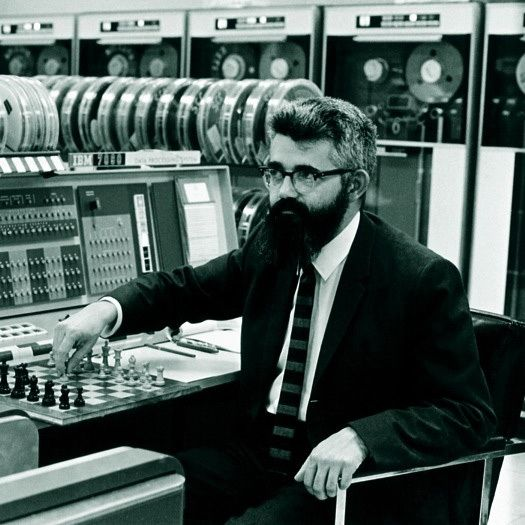
\includegraphics[height=1in]{img/mccarthy.jpg}
  \end{center}
  \begin{itemize}
    \item Church’s lambda calculus was based on simple rules.
    \item In the 1950’s, John McCarthy created \emph{Lisp}, the first functional programming language.
    \item McCarthy is also famous for coining the term \emph{artificial intelligence}.
    \item Easy to write an interpreter -- many dialects similar to Lisp, like Scheme and Racket.
  \end{itemize}
\end{frame}


\begin{frame}{Expressions in $\lambda$-calculus}
  Programs in Lisp are like $\lambda$-calculus expressions. Every expression is either:
  \begin{description}
    \item[$x$] a variable
    \item[$(M N)$] an application
    \item[$\lambda x.M$] an abstraction
  \end{description}
\end{frame}


\begin{frame}{Why study functional programming?}
  \begin{itemize}
    \item Functional programming languages and ideas have had a resurgence in the last few years.
    \item One reason is that functional programming lends itself to parallel programming.
    \item Another reason is that artificial intelligence has its roots in functional programming.
    \item The main reason to learn it is because it makes you think about what programming is, or even better, what computation is.
    \item Note that a lot of imperative programming languages have recently reverse engineered functional ideas.
  \end{itemize}
\end{frame}

\begin{frame}{Some concepts for further discussion}
  \begin{itemize}
    \item Anonymous functions
    \item First class functions
    \item Higher order functions
    \item Side effects
    \item Recursion
    \item Map and reduce
  \end{itemize}
\end{frame}









 
\end{document}
 